\begin{fact} \label{iso-tri}
	Considérons tous les triangles de périmètre fixé $p$. Parmi tous ces triangles, il en existe un seul d'aire maximale, c'est le triangle équilatéral de côté $c = \dfrac13 p$.
\end{fact}


\begin{proof}	
	Nous allons donner une démonstration constructive via une application itérative du fait \ref{tri-one-side-fixed} donnant, par passage à la limite, le triangle équilatéral d'aire maximale, et ceci avec une vitesse de convergence exponentielle.%
	\footnote{
		Ceci ne va nécessiter que l'emploi de propriétés simples de l'ensemble des réels.
	}
	Partons donc d'un triangle $ABC$ quelconque, mais de périmètre $p$, le fait \ref{tri-one-side-fixed} donne successivement les triangles $ACD$, $ADE$, $AEF$ et $AFG$ isocèles en $D$, $E$, $F$ et  $G$ respectivement, ayant tous pour périmètre $p$, et ceci avec des aires de plus en plus grandes.  
	Le dessin suivant amène à conjecturer qu'en poursuivant ce procédé de construction, nous aboutirons \focus{à la limite} à un triangle équilatéral.

	\begin{center}
		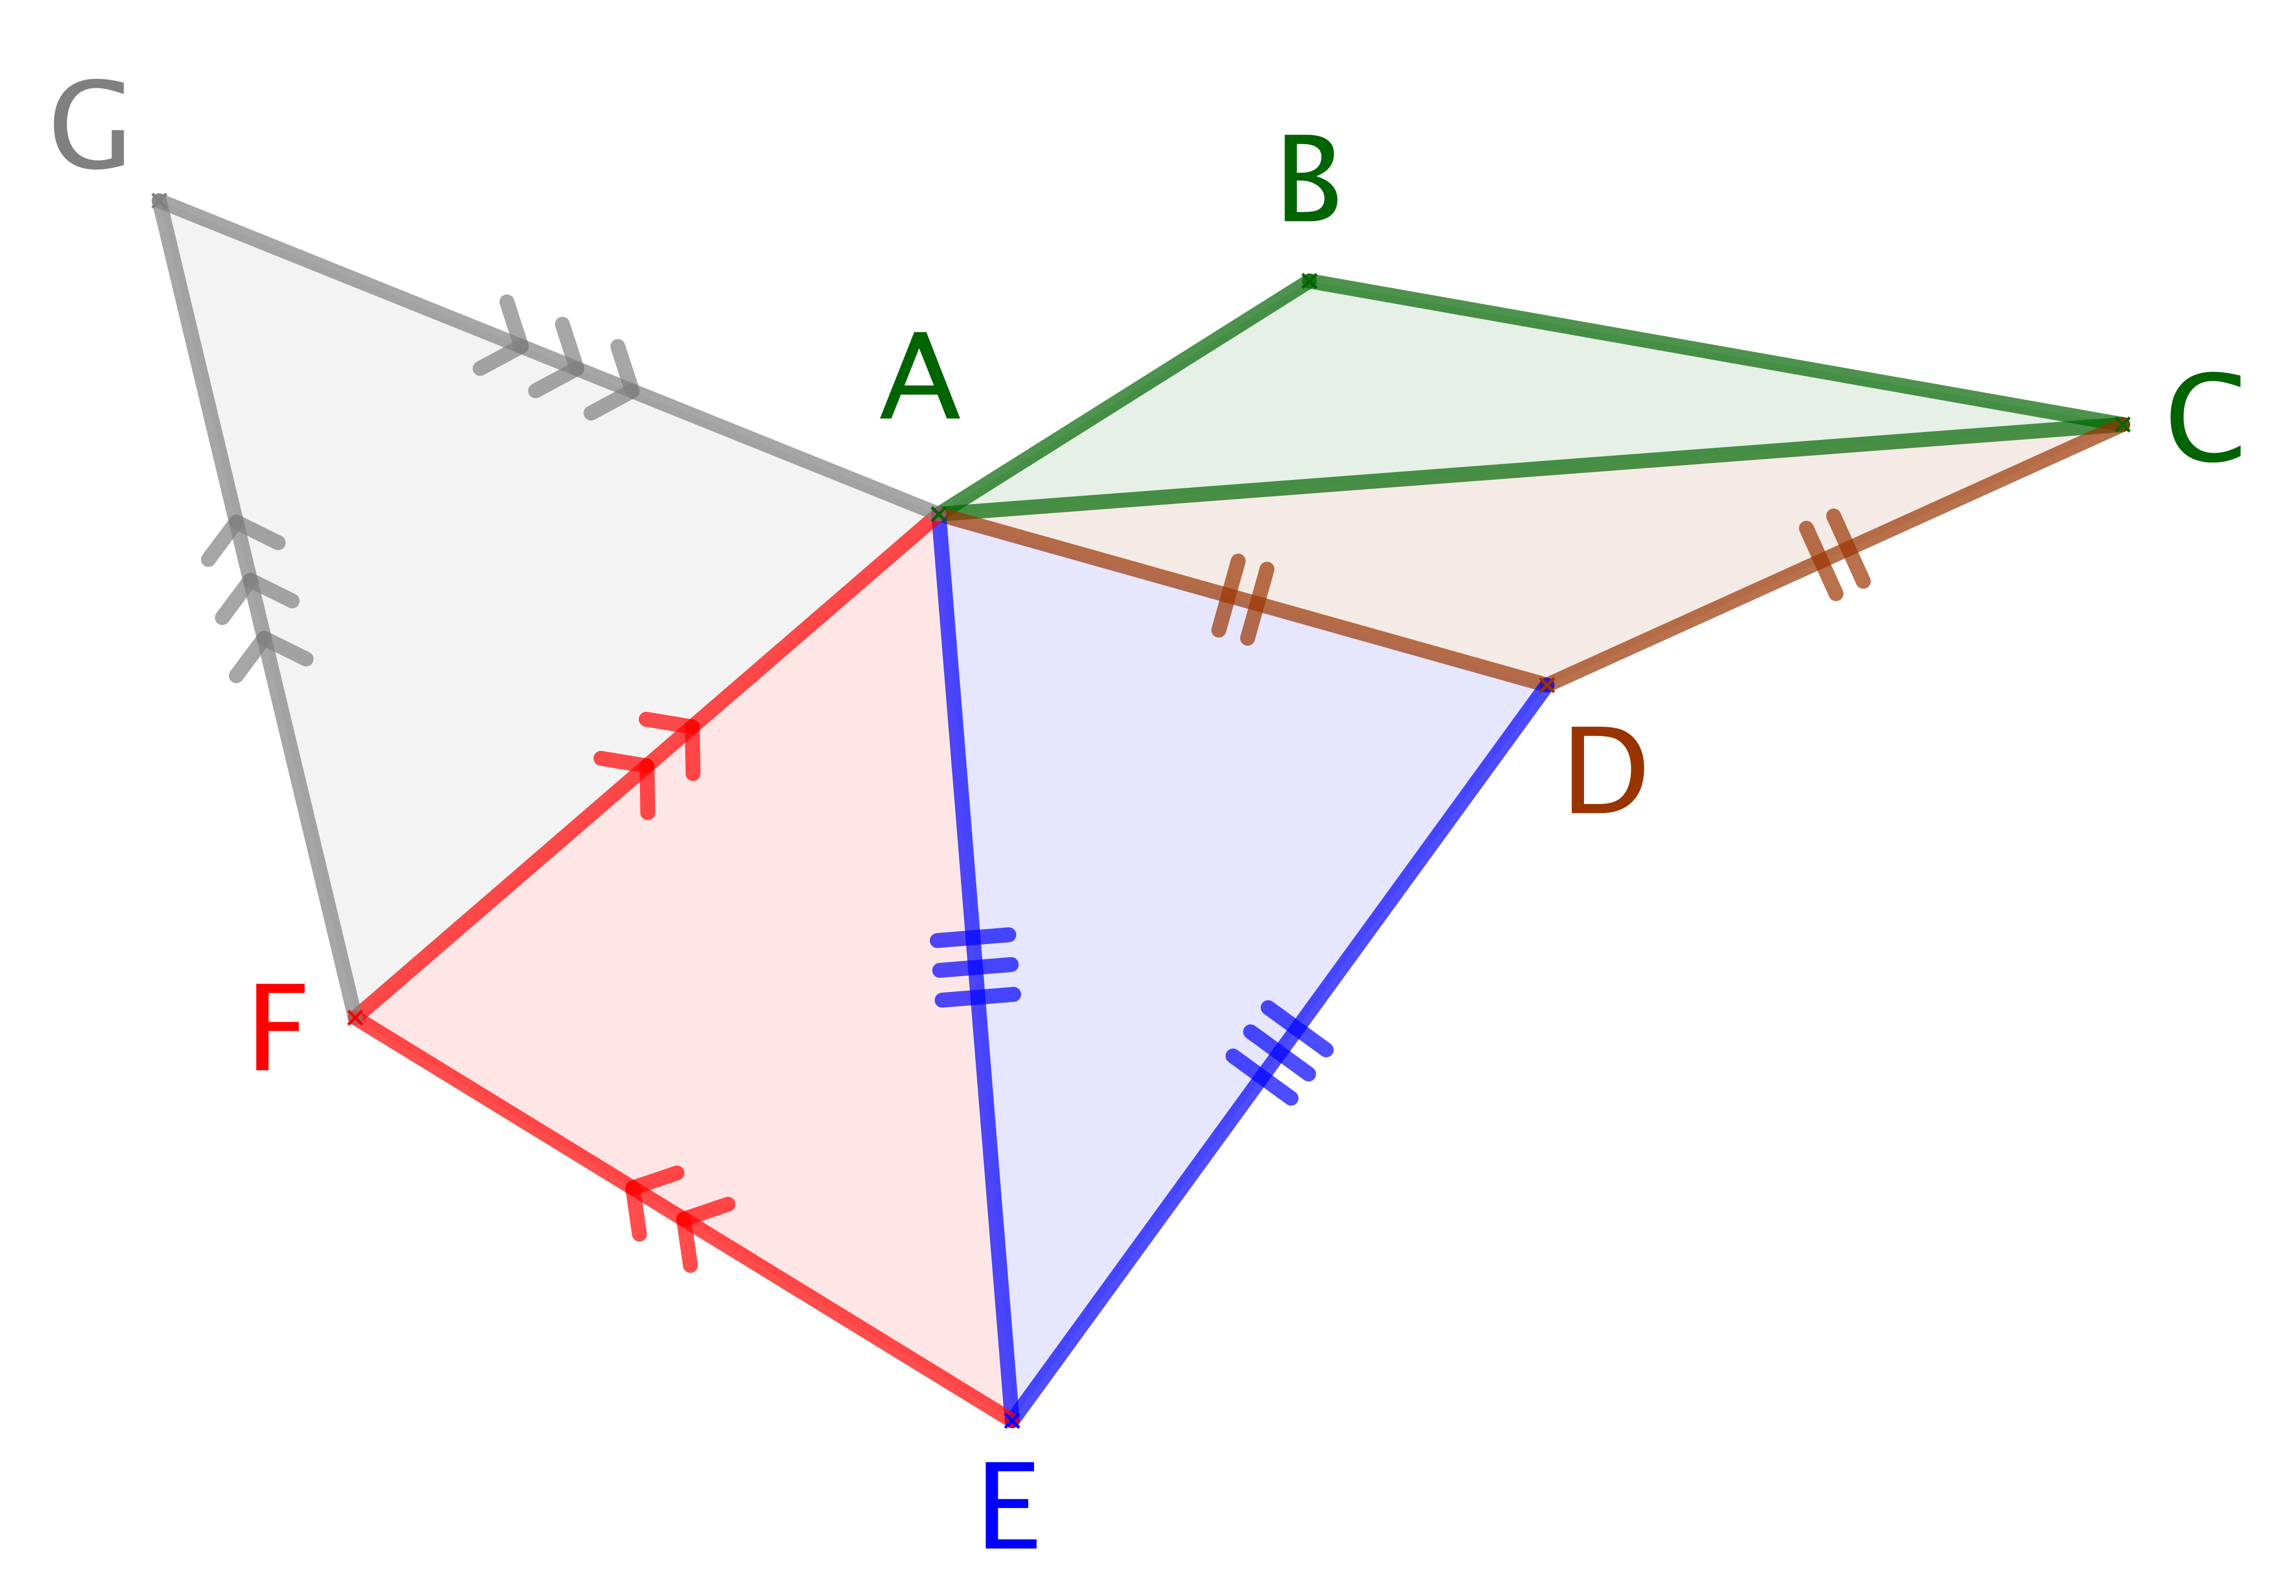
\includegraphics[scale=.4]{content/triangle-gene/proof.png}
	\end{center} 

	
	Le passage du triangle initial $ABC$ au 1\ier\ triangle $ACD$ isocèle en $D$ nous amène à nous concentrer sur ce que donne notre procédé d'agrandissement d'aire à périmètre fixé pour des triangles isocèles. 
	Voici ce que nous pouvons affirmer en supposant $AC > AD$, comme dans notre exemple (nous allons voir que cette hypothèse est sans conséquence).
	%
	\begin{enumerate}
		\item Comme $AC + 2 AD = p$ et $AC > AD$, nous avons $AC > \frac13 p > AD$.
		À l'étape suivante, comme $AD + 2 AE = p$, nous obtenons nécessaireemnt $AD < \frac13 p < AE$.


		\item Pour $AEF$ isocèle en $F$, comme $AE + 2AF = p$, nous arrivons à  $AE > \frac13 p > AF$.
		
		
		\item \label{tri-equi-conv}
		Tentons de quantifier les écarts à la mesure pivot $p^{\,\prime} = \frac13 p$. 
		%
		\begin{itemize}
			\item Dans $ACD$, posant $AD = p^{\,\prime} - \epsilon_1$, nous avons $AC = p^{\,\prime} + 2 \epsilon_1$.

			\item Dans $ADE$, posant $AE = p^{\,\prime} + \epsilon_2$, nous avons $AD = p^{\,\prime} - 2 \epsilon_2$.

			\item Dans $AEF$, posant $AF = p^{\,\prime} - \epsilon_3$, nous avons $AE = p^{\,\prime} + 2 \epsilon_3$.

			\item Dans $AFG$, posant $AG = p^{\,\prime} + \epsilon_4$, nous avons $AF = p^{\,\prime} - 2 \epsilon_4$.

			\item Donc
			$\epsilon_2 = \frac12 \epsilon_1$,
			$\epsilon_3 = \frac12 \epsilon_2$
			et
			$\epsilon_4 = \frac12 \epsilon_3$.
		\end{itemize}
	\end{enumerate}


	\smallskip
	
	Voici les enseignements de ce qui précède en partant d'un triangle $ABC$ non équilatéral.
	%
	\begin{itemize}
		\item Si $AC = \frac13p$, dès la 1\iere\ itération, nous avons un triangle équilatéral d'aire plus grande.
		
		
		\item Si $AC \neq \frac13p$, notre procédé n'arrivera jamais en un nombre fini d'étapes à un triangle équilatéral.
		Dans ce cas, le point \ref{tri-equi-conv} ci-dessus nous donne une convergence exponentielle des longueurs des côtés vers $p^{\,\prime} = \frac13 p$, tout en ayant des aires des plus en plus grandes.
	\end{itemize}
	
	Dans tous les cas, l'aire d'un triangle non équilatéral de périmètre $p$ est strictement majorée par celle du triangle équilatéral de périmètre $p$. Et tout ceci a été obtenu via de la géométrie et de l'analyse élémentaires!
\end{proof}
